\subsection{Robustness and generalisation}\label{sec:robust}
Finally, we evaluated all policies \emph{zero-shot}, without retraining or re-tuning, under shifted conditions: different levels of sensor noise at test time, resilient and fatigue-prone worker profiles, and lighter or heavier workloads (Fig.~\ref{fig:robust}; full results in Supplementary Table~S4). We also trained five seeds of a domain-randomised agent (AA-DQN-DR) on randomly sampled workloads ($N\in\{8,\dots,16\}$), worker profiles ($\pm30\%$ on all rate parameters) and noise levels ($\sigma_o\in[0.05,0.2]$).

\emph{Sensor noise.} Both AA-DQN variants are insensitive to the test-time noise level. Their returns vary by less than 0.15 between $\sigma_o=0$ and $\sigma_o=0.3$ (primary 12.14--12.27, intensity-only 12.57--12.71). The threshold rules, in contrast, degrade as noise grows, because spurious threshold crossings trigger unnecessary breaks. SPT-Threshold falls from 12.30 to 11.35 and from 71.4\% to 65.6\% on-time, and EDF-Threshold falls from 11.35 to 9.63. The periodic rules are unaffected, because they ignore the cognitive signals altogether. Learned policies therefore degrade more gracefully than reactive rules when state estimation is poor. Their history-based estimate averages out noise that a threshold applied to a single reading cannot.

\emph{Worker profiles.} The ranking depends on the profile. For fatigue-prone workers, the learned policies (primary 10.05, intensity-only 10.40) and the SPT-based rules (10.21--10.59) form the leading group, far ahead of the EDF-based rules (7.5--7.9). For resilient workers, who need less rest, the EDF-based rules attain the highest return (EDF-Periodic 15.01), with the intensity-only agent close behind (14.76) and achieving the highest on-time rate (81.1\%). No single policy is best for every profile, which argues for personalisation (Section~\ref{sec:future}).

\emph{Workload.} Generalisation to different numbers of tasks per day is the clearest weakness of the learned policies. With 8 tasks per day the threshold rules complete almost all tasks on time and outperform the agents (EDF-Threshold 13.12 versus 11.71--12.20). With 16 tasks the SPT-based rules are best (SPT-Threshold 11.61 versus 9.69--10.03). Although the observation is normalised by $N$, the queue statistics of these days lie outside the training distribution. Domain randomisation improved the 16-task result (10.35) and kept on-time rates close to the nominally trained agent across conditions, but it did not close the gap and lowered nominal performance (11.63). A simple randomisation over conditions with checkpoint selection on nominal days is therefore insufficient. Workload-aware training curricula or explicit conditioning on the workload level are needed for deployment across heterogeneous workloads.

\begin{figure}[!htbp]
\centering
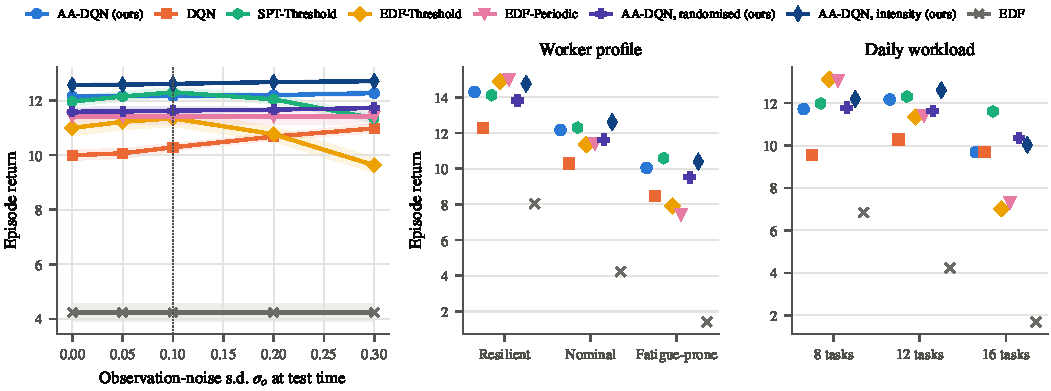
\includegraphics[width=\textwidth]{figures/fig_robustness.pdf}
\caption{Zero-shot robustness. Left: return versus test-time observation noise (training/tuning at $\sigma_o=0.1$, dotted line; shaded: 95\% CIs). Centre and right: return for different worker profiles and daily workloads. Heuristics use parameters tuned in the nominal environment.}
\label{fig:robust}
\end{figure}
